\documentclass[conference]{IEEEtran}

\IEEEoverridecommandlockouts
\usepackage{cite}
\usepackage{amsmath,amssymb,amsfonts}
\usepackage{algorithmic}
\usepackage{graphicx}
\usepackage{textcomp}
\usepackage{xcolor}
\usepackage{fancyhdr}
\usepackage{lipsum}% generate text for the example

\def\BibTeX{{\rm B\kern-.05em{\sc i\kern-.025em b}\kern-.08em
    T\kern-.1667em\lower.7ex\hbox{E}\kern-.125emX}}
    
\fancypagestyle{firstpagefooter}{%
  \fancyhf{}
  \renewcommand\headrulewidth{0pt}
  \fancyfoot[R]{Forced-Directed List-Scheduling, Hamm-Lippstadt Hochschule}
}

\pagestyle{empty}

\begin{document}
\title{Forced-Directed List-Scheduling}

\author{\IEEEauthorblockN{Vytaras Juraska}
\IEEEauthorblockA{\textit{Electronics Engineering (6\textsuperscript{th} Semester)} \\
\textit{Hamm-Lippstadt Hochschule}\\
Lippstadt, Germany \\
vytaras.juraska@stud.hshl.de}
}

\maketitle

\begin{abstract}
an explanation and a deep dive on the working concept, the history of development and the usage of a very specific extension of an already existent algorithm. Understanding and analyzing the relevancy and connection when applying specified algorithm to the current time and age technology standards.
\end{abstract}


%\begin{IEEEkeywords}
%component, formatting, style, styling, insert
%\end{IEEEkeywords}

\thispagestyle{firstpagefooter}

\section{Introduction}
This specific scheduling algorithm is essentially an extension of an already existent scheduling algorithm - Forced-Directed scheduling. It adds an extension of List-scheduling to the mentioned algorithm. It was created to have the most optimal solution for a scheduling problem, where both resources and the latency of the operations is constrained.

\textbf{NOTE}
Throughout the explanation of Force-Direct and Force-Direct List-Scheduling algorithms, the references ([1] and [2]) are using this specific sequencing diagram (Figure \ref{sequence}).

\begin{figure}[htbp]
\centerline{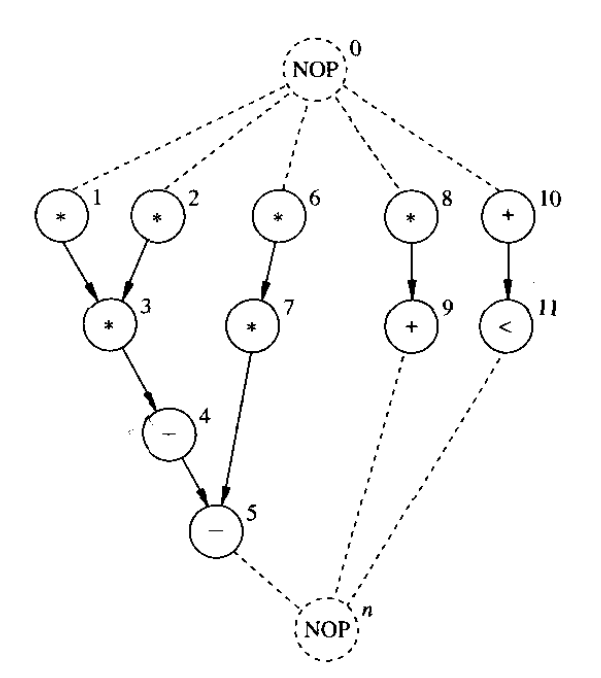
\includegraphics[scale=.5]{Sequencing_Graph.png}}
\caption{Initial Sequencing Graph}
\label{sequence}
\end{figure}

\subsection{Force-Direct Relevant Part}
Force-Directed scheduling algorithm was created to find the most optimal and sufficient approach on how to solve resource and latency constrained (limited) scheduling problems. Visually it is, in a sense, where each of it's components have a force, which is pushing each component away from each other, creating a natural distance between each other, with a corresponding length (Figure \ref{fdlayout}).

\begin{figure}[htbp]
\centerline{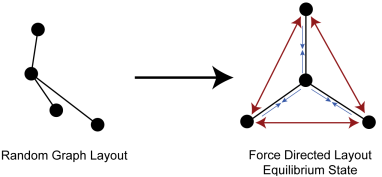
\includegraphics[scale=.5]{force_directed_layout_example.png}}
\caption{Force-Directed visual layout example}
\label{fdlayout}
\end{figure}

Considering how the Forced-Directed List-Scheduling works, we have to understand the basics of Forced-Directed algorithm. The time constrain has two variables, the earliest time variable and the latest time variable when the operation is expected to be executed, both of the variable form a, so called, time frame. This concept has been taken from and can be calculated with ASAP (As Soon As Possible) and ALAP (As Late As Possible) algorithms.

Probability of operations is defined as follows: outside the time frame it is zero, inside the time frame, it is the reciprocal of the frame width. Hence the larger the width of the time frame, the lower the probability is for scheduled operation to be successfully executed in the corresponding time step. So in this specific algorithm, it is required to not only have a limited time frame, but also the most optimal solution is to keep the time frame as narrow as possible.

\textbf{NOTE} Further explanation would lead to the first example of Force-Direct Scheduling calculations, the example refers to Initial Sequencing Graph. It's time distribution graph for the components in the exercise (Figure \ref{fdexample}).

\begin{figure}[htbp]
\centerline{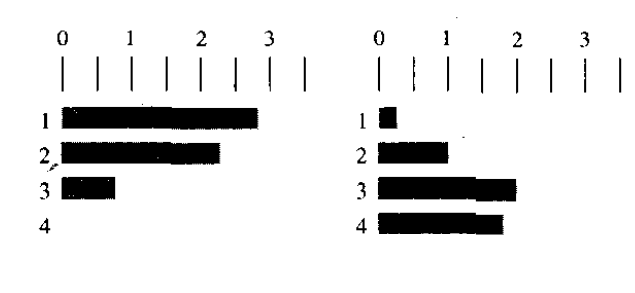
\includegraphics[scale=.5]{Example5.4.10.png}}
\caption{Distribution graph for multiplexer and ALU}
\label{fdexample}
\end{figure}

\subsection{List-Scheduling Relevant Part}
Relatively simple explanation of List-Scheduling is giving some sort of property to each of the component and defining a position of the component in the list corresponding to it properties unit.

\subsection{Force-Direct List-Scheduling}
As mentioned in the Force-Direct algorithm introduction, this specific solution is an addition of List-Scheduling to previously mentioned algorithm. The conditions of the problem are similar to Force-Direct algorithm's, a limited and minimal time frame of the operation, caused by the fixed hardware constrains.

Force-Direct used to figure out the priority of each process 

\section{History of Development}
A detailed timeline of how this method came to be developed

\section{Usage and Appliance}
Where is it applied in real situations, where is it used in

\textbf{NOTE} In the [2] reference, and in the other various resources this specific graph was displayed as a common comparison figure for FDLS. Referenced description - Fifht-Order Digital Elliptical Wave Filter (Figure \ref{wavefilter}) (sounds like a tongue twister).

\begin{figure}[htbp]
\centerline{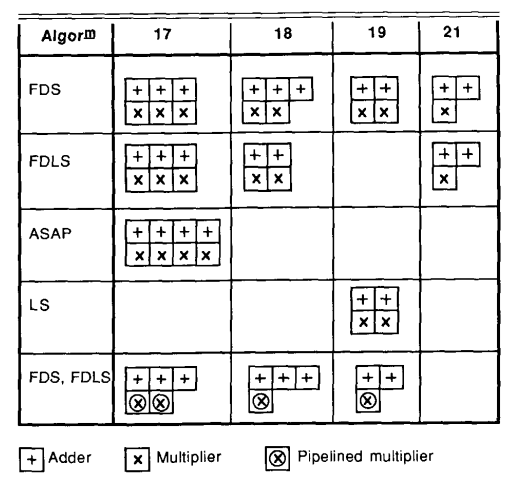
\includegraphics[scale=.5]{Result_Applience.png}}
\caption{}
\label{wavefilter}
\end{figure}

\section{Advantages}
Any positive advantages related to this method, why is it useful to use this method

\section{Disadvantages}
Any disadvantages, which might lead to certain issues, where this method can not be applied

\section{Evaluation}
Personal opinion, is it useful, is there future for this method?

\section{Conclusion}
Final thoughts, concluding the topic

\begin{thebibliography}{00}
\bibitem{b1} 
Giovanni De Micheli "Synthesis and Optimization of Digital Circuits"
\bibitem{b2} 
P. G. Paulin and J. P. Knight, "Force-directed scheduling for the behavioral synthesis of ASICs,"
\end{thebibliography}

\end{document}
